\chapter{Social Routing Client Application}
The Social Routing Client Application is composed by four major components, each with it's own compromise and objective.
The Activities\cite{activities} and Fragments\cite{fragments} to represent the User Interface (UI) where the user can interact with the application, the 
View Models\cite{viewmodel} to store and manage UI related data, a Repository that handles data operations and knows where to retrieve data from and a 
Remote Data Source to communicate with external components, for instance the Social Routing API, the Google Sign In API\cite{googlesignindocs} or Google Maps Platform. 
This logic is represented in the figure \ref{fig:clientarchitecture}.

\begin{figure}[h]            
        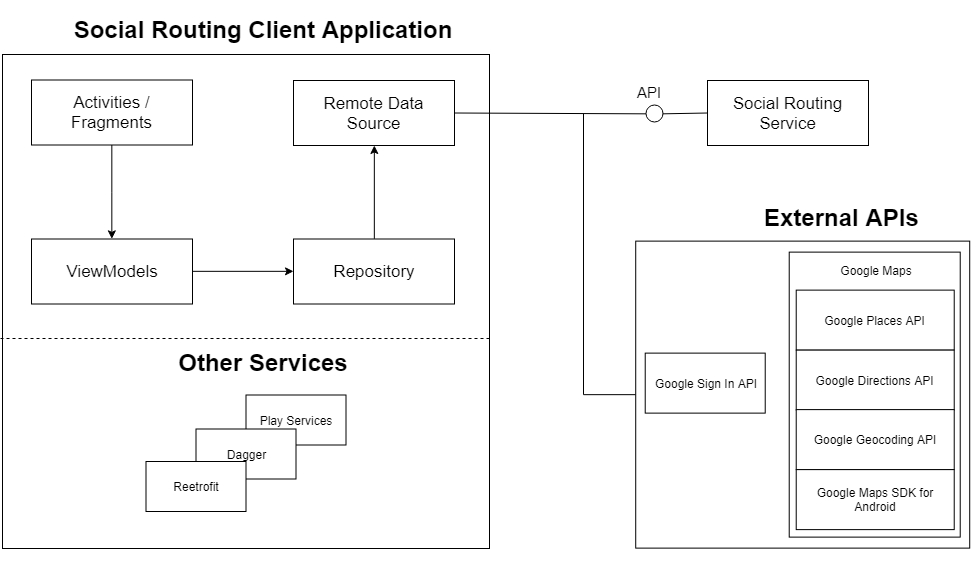
\includegraphics[width=\textwidth]{images/project-structure/social-routing-client-application-structure.PNG}
        \caption{Social Routing Client architecture.}
        \label{fig:clientarchitecture}
\end{figure}
\newpage

\section*{Remote Data Source}
Module that has the objective of communicating with external APIs which it does by executing requests to either the Social Routing API, the Google Maps Platform or the Google Sign In API. 
The Component knows the structure of the HTTP request to the endpoints, like the parameters and meta-data necessary to obtain the required Response. After the request is done, the webservers\cite{webserver} 
provide the response in the Json\cite{jsonwebsite} format, however the response is deserialized using the library Jackson\cite{jackson}, to convert it to Object. 
So was defined all the input model objects, to automatically deserialize the response to object.\\

\section*{Repository}
The Repository Handles data operations, knows where to get the data from
and what API calls to make when the data is updated. A repository can be
considered a mediator between different data sources, such as web services. \\
The application has repositories specified to the Social Routing API and another to Google Maps Platform, which contains
multiple APIs. Each one as correspondent Web Service that uses the
framework Retrofit\cite{retrofit}, used to make a synchronous or asynchronous HTTP request to the remote webserver. The Repository obtains the data
from the web server and can only have two possible request status: Failure or Success. It returns the data contained in a LiveData\cite{livedata} because when the data 
updates can then be observable. \\
The Repository specific to our API (Social Routing API) knows all the endpoints\cite{endpoint TODO} that should make the request by doing a request to the root endpoint, 
depending on the objective and the functionality, like the endpoints to sign in, to get user info, routes, create a route, get all categories, update a route, amongst others. \\
On the other hand the other repository is used to make request to the Google Webserver (Google Maps Platform) about the geocode\cite{geocode} of a location, the directions to a 
coordinate in the map and the places of a given area. 

\section*{View Models}
Component used when the UI experiences a change. The View Model calls
other components to load the data, and it can forward user requests to
modify the data however it doesn't know about UI components, 
it is completely separated from them. \\
This component has a simple implementation, the application contains three View Models one for the Routes information (get, creation, update, search), 
to the User (get, update) and another to the Google Maps Platform (information of a location, places, directions). It uses the repository to obtain the data and 
then return it in the shape of Livedata.

\section*{Activities/Fragments}
The only concern of this component is to provide a way for the user to interact with the application and with the view.
All activities extend a BaseActivity that has a global behavior such as when the data is changed, is necessary to update the view and to show some view components 
like a toast\cite{toasts}, progress bar\cite{progressBar} or even start another activity, to be more noticeable to the user what is happening on the application.\\

Each Activity has its own :
\begin{itemize}
        \item Design: defined by one or more layouts that contains buttons, images, input text, fragments (for instance the map fragment provided by Google), 
        with which the user can interact and make actions.
        \item Behavior: when the data changes the view needs to be updated, behavior this, that is defined with either a success or error, using the ViewModel.
\end{itemize}

\subsection*{BaseActivity}
\begin{itemize}
        \item Design: No layout.
        \item Behavior: Is a abstract implementation of a Activity, where contains generic behavior to view components and knows how to handle changes in the Livedata from View Model, 
        to all the Activities that implement it.
\end{itemize}

\subsection*{LoginActivity}
\begin{itemize}
        \item Design: Login Activity Layout.\cite{loginactivitylayout}
        \item Behavior: Where the Authentication\ref{authentication} happens, using the google account credentials the user can login/authenticate in the server side and a
request to the Root endpoint of the Social Routing API is done.
\end{itemize}

\subsection*{NavigationActivity}
\begin{itemize}
        \item Design: Navigation Activity Layout.\cite{navigationactivitylayout}
        \item Behavior: The client can navigate through the application functionalities with this activity. This layout contains a text box to input the location, to search for the best 
route possible, a list that shows the closest routes of the user current location, doing a request to the Social Routing Service with the default filters like all categories,
a route with short duration and finally a panel that contains buttons to go to other activities, like RouteCreationActivity\ref{routecreationactivity} and 
UserProfileActivity\ref{userprofileactivity}.
\end{itemize}
\newpage

\subsection*{RouteCreationActivity} \label{routecreationactivity}
\begin{itemize}
        \item Design: Route Creation Activity Layout.\cite{routecreationactivitylayout}
        \item Behavior: A core functionality of the Social Routing Client Application is in this activity, because is where the user can create a route and it's corresponding metadata.
        Initially is obtained asynchronously a Fragment, provided by Google Play Service\cite{googleplayservices}, that represents the Google Maps\cite{googlemaps} and right after the map is RouteDetailsActivity
        a form pops up asking for the desired location of the route, to be created. After the user inputs the location name, is made a request to Geocoding API\cite{geocodingapi} from google to obtain 
        the geocoordinates to do a zoom in the map. Then request the user can click in the map to select the route points, to create the path and are saved. When the route path is 
        finished, the user click must click in the button continue to proceed to the Places of interest, that is, is made a request to Google Places API\cite{googleplacesapi} to obtain the Places Of interest
        near of the route points (in a range of one hundred meters) that can be added as metadata of the route. To conclude, is necessary to fill a form, in the RouteCreationMetadataActivity
        \ref{routecreationmetadataactivity} to terminate the creation.
\end{itemize}

\subsection*{RouteCreationMetadataActivity} \label{routecreationmetadataactivity}
\begin{itemize}
        \item Design: Route Creation Metadata Layout.\cite{routecreationametadatactivitylayout}
        \item Behavior: The objective of this activity is the termination of the route creation. Where receives the route information that was obtained from the previous activity (RouteCreationActivity\ref{routecreationactivity})
        via Intent \cite{intent} and is needed to fill fields about the route like the name, description, categories, duration and image to fully create the route and make a POST 
        request to the Social Routing Service to be created, if is succeeded is shown the route representation in the RouteRepresentationActivity\ref{routerepresentationactivity}.
\end{itemize}

\subsection*{RouteDetailsActivity}
\begin{itemize}
        \item Design: Route Details Activity Layout.\cite{routedetailsactivitylayout}
        \item Behavior: Activity to represent some metadata of the route like the name, description, categories, duration and image that are obtained via Intent and are represented to the 
        layout.
\end{itemize}

\subsection*{RouteRepresentationActivity} \label{routerepresentationactivity}
\begin{itemize}
        \item Design: Route Representation Activity Layout.\cite{routerepresentationactivitylayout}
        \item Behavior: Through Intent is sent the route Url\cite{url} to this activity, to do a request to Social Routing Service and obtain all the route detailed information. The Google Maps
        is initialized and is shown to the user the route path with blue markers and lines that are drawn in the map and the places of interest with red markers.
\end{itemize}
\newpage

\subsection*{RouteSearchActivity}
\begin{itemize}
        \item Design: Route Search Activity Layout.\cite{routesearchactivitylayout}
        \item Behavior: The Search functionality is done with specific filters (categories, duration and location) and it is done in this activity, by passing the correspondent parameters to it
        and is made a request to Social Routing API, if succeeded are shown in a list the results.
\end{itemize}

\subsection*{UserProfileActivity} \label{userprofileactivity}
\begin{itemize}
        \item Design: User Profile Activity Layout.\cite{userprofilectivitylayout}
        \item Behavior: Previously was done a request to the root endpoint to obtain the Urls of the API and also comes the user profile Url of the user authenticated and is used to make 
a request to obtain all the information about it.
\end{itemize}

The Client Application has the minimum API level 23 and the target API level is 28, so the Platform version is the Android 9.
It uses Kotlin as the only the programming language in the project which is an object oriented programming language. 
The goal was to improve the coding experience in a way that was practical and effectual. Kotlin is entirely compatible with Java and was specifically designed
to improve existing Java models by offering solutions to API design deficiencies. \\
The core functionalities of the application require a map to create the routes and to show them which was done was using the Google Maps Platform.
All the functionalities of the application are provided from de Social Routing Service, except all that is related to the Google Maps. All the information is obtained from the server by doing
requests to the correspondent endpoint and it is always necessary to send either the token created by the server or the Google Sign-In API tokenId, used on the user registration process.
The requests that are related to location retrieval or Map UI require a specific request to the Google Maps API. \\
\newpage
\section*{Use Case}
As an example, the user first experience flow of the application is the following:
        \begin{itemize}
                \item The user provides his google account credentials to authenticate with the application, which in its turn makes a request to the backend server.
                \item The user will be redirected to a navigation screen that contains a route search bar and a left panel menu with buttons to redirect to the screens of user profile and route creation.
                \item After the user searches routes using a location, a redirection to a new screen occurs in which a list of found routes is shown.
                \item Once a route is chosen and pressed upon, a new activity with a map is shown, where the route is represented and with a button to start Live Tracking.
                \item By choosing to start Live Tracking the user location is now showed as well as a path to reach the beginning of the chosen route.
                \item If the user wants to see the his profile he may go back until the navigation screen and click in the left panel and then in the User Profile button.
                \item In the user profile the user information (user rating, name, email and routes created) is shown.
                \item For creating a route, a button press in the bar menu is required.
                \item This action takes the user to a new screen that shows the map, a button to finish and a form, asking the location of the route that will be created.
                \item The user must then insert the location on which the map will zoom in.
                \item A click in the map will add the pressed location point to the route being created. If something wrong occurs the user can delete the last point of the route clicking the button on the top of the screen.
                \item When finished the user click in the button to fill the final form that contains the name, description and category of the route.
        \end{itemize}

\section*{Internal Services}


\section*{External Services}


\section*{Authentication} \label{authentication}